\chapter{Key escrow server}\label{escrow}
Before Tang, automated decryption was usually handled by Key Escrow server (also known as a “fair” cryptosystem).
A client using Key Escrow usually generates a key, encrypts data with it and then stores the key encryption key on a remote server.
However, it is not as simple as it sounds and there are couple of security concerns.

\section{Escrow security}

To deliver these keys we want to store on Escrow server, we have to encrypt the channel on which we distribute them.
When transmitting keys over non secure network without encrypted link, anyone listening to the network traffic could immadiately fetch the key.
This should signal security risks, and, of course, we do not want any third party to access our secret data.
Usually we encrypt a channel with TLS(Transport Layer Security) or GSSAPI (Generic Security Services Application Program Interface) as shown on a Figure \ref{fig:escrowmodel} below.
Unfortunatelly, this is not enough to call the communication secure.

We cannot just start sending these keys to the escrow server, if we do not know whether this server is the one it acts to be.
This server has to have its own identity to be verified, and the client have to authenticate to this server too.
Increasing amount of keys implicates a need for Certification Authority server (CA) or Key Distribution Center (KDC) to manage all of them.
With all these keys, and at this point only, server can verify if the client is permitted to get their key, and the client is able to identify trusted server.
This is a fully stateful process.
To sum up, an authorized third party may gain access to keys stored on Escrow server under certain circumstances only.

\begin{figure}[h]
    \centering
    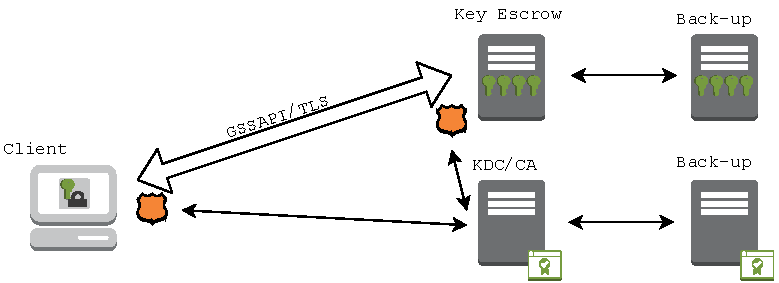
\includegraphics[scale=0.7]{figures/EscrowModel.pdf}
    \caption{Escrow model}
    \label{fig:escrowmodel}
\end{figure}

Complexity of this system increases the attack surface and for this complex system it would be unimaginable not to have backups.
Escrow server may store lots of keys from lots of different places and basically we can not afford to lose them.
\todo{refactor chapter; add more info}
